% LTeX: language=it
% LTeX: enabled=false
\documentclass{beamer}

\mode<presentation>
{
	\usetheme[
		titlepagelogo=logo_verticale_BLACK.png,
		language=italian,
		coding=utf8,
		bullet=square,
		pageofpages=di,
		color=green,
		secondsupervisor=true,
	]{TorinoTh}
	
}

\usepackage[italian]{babel}
\usepackage{mathtools}
\usepackage{mleftright}

\mleftright

\newcommand{\spacedmiddle}[1]{\mathrel{}\middle#1\mathrel{}}
\newcommand{\ket}[1]{\left | #1 \right \rangle}
\newcommand{\conf}{\mathfrak{C}_{M}}
\newcommand{\hil}{\ell^{2}}
\newcommand{\hiluninorm}{\hil_{1}}
\newcommand{\Zero}{\alert{\mathbf{0}}}
\newcommand{\One}{\alert{\mathbf{1}}}

% LTeX: enabled=true
\title
{Macchine di Turing Quantistiche}

\author
{Pietro Zignaigo}

\institute
{Università di Genova}

\rel
{Elena Zucca}
\secondsupervisor
{Francesco Dagnino}

\date
{16-12-2024}

\subject
{Macchine di Turing Quantistiche}

\begin{document}

\begin{frame}
	\titlepage
\end{frame}

\begin{frame}
	\tableofcontents[hideallsubsections]
\end{frame}

\section{Introduzione}

\subsection{Computazione quantistica}

\begin{frame}{\subsecname}{}
	\begin{itemize}
		\item<1-> Informazione in un computer quantistico =\\
		sovrapposizione di stati discreti
		\item<2-> Unità minima di informazione quantistica: \alert{qubit}
	\end{itemize}
	\begin{align*}
			\onslide<2->{1 \ket{\Zero} + 0 \ket{\One}
			&\qquad  0 \ket{\Zero} +  1 \ket{\One} \\\\}
			\onslide<3->{\frac{1}{\sqrt{2}} \ket{\Zero} + \frac{1}{\sqrt{2}} \ket{\One}
			&\qquad \frac{1}{\sqrt{2}} \ket{\Zero} + i \frac{1}{\sqrt{2}} \ket{\One}}
	\end{align*}
\end{frame}

\begin{frame}{\subsecname}{}
	\begin{itemize}
		\item<+-> Osservazione:
		\begin{itemize}
			\item Si ottiene 1 o 0
			\item Probabilità dipendente dai pesi
			\item Collasso su \( \ket{\Zero} \) o su \( \ket{\One} \)
		\end{itemize}
		\item<+-> \foreignlanguage{english}{Quantum advantage}: per certi problemi, \\
		complessità temporale algoritmi quantistici \(<\) \\
		complessità temporale algoritmi classici
	\end{itemize}
\end{frame}

\subsection{Modello matematico}

\begin{frame}{\subsecname}{Spazi di Hilbert}
	\begin{itemize}
		\item<+-> \alert{Spazio di Hilbert} generato da \( \mathcal{B} \)
		\[ \hil \left ( \mathcal{B} \right ) = \left \{ \phi : \mathcal{B} \rightarrow \mathbb{C} \spacedmiddle | \left \| \phi \right \|^{2} = \sum_{\mathcal{C} \in \mathcal{B}} \left | \phi \left ( \mathcal{C} \right ) \right |^{2} < \infty \right \}\]
		\item<+-> Prendiamo in considerazione solo \(\hiluninorm\)
		\[ \hiluninorm \left ( \mathcal{B} \right ) = \left \{ \phi \in \hil \left ( \mathcal{B} \right ) \spacedmiddle | \left \| \phi \right \|^{2} = 1 \right \}\]
	\end{itemize}
\end{frame}

\begin{frame}{\subsecname}{Operatori}
	\begin{itemize}
		\item<+-> Trasformazione stato quantistico = operatore lineare = \\
		matrice \( \#\mathcal{B} \times \#\mathcal{B} \)
		\item<+-> Possono essere usati solo \alert{operatori unitari}
		\begin{itemize}
			\item invertibili \(\rightarrow\) meccanica quantistica è reversibile
			\item conservano la norma \(\rightarrow\) per rimanere in \(\hiluninorm \left ( \mathcal{B} \right )\)
		\end{itemize}
		\item<+-> Unitarietà in forma matriciale
		\begin{itemize}
			\item Colonne con norma 1 (per conservare la norma)
			\item Ogni coppia di colonne deve essere ortogonale
		\end{itemize}
	\end{itemize}
\end{frame}

\subsection{Macchina di Turing}

\begin{frame}{\subsecname}{}
	\centering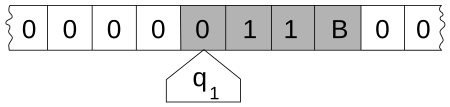
\includegraphics[width=6.5cm]{Turing_machine_2b.png}
	\begin{itemize}
		\item<+-> Modello matematico per descrivere tutti gli algoritmi
		\item<+-> \alert{Funzioni calcolabili}: Funzioni parziali \( f : \mathbb{N} \rightarrow \mathbb{N} \) modellabili da una macchina di Turing
	\end{itemize}
\end{frame}

\section{Macchina di Turing quantistica}

\subsection{Configurazioni}

\begin{frame}[t]{\subsecname}{}
	\centering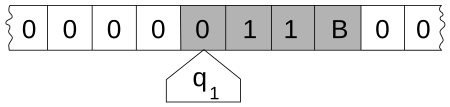
\includegraphics[width=6.5cm]{Turing_machine_2b.png}\\
	\only<1,2>{
		\alert{Configurazione} di una macchina di Turing
		\[ \left \langle \alpha, q, \beta, i \right \rangle \in \Sigma^{*} \times \mathcal{Q} \times \Sigma^{*} \times \mathbb{Z} \]
	}
	\only<2->{
		\[ \conf = \Sigma^{*} \times \mathcal{Q} \times \Sigma^{*} \times \mathbb{Z} \times \mathbb{N} \]
	}
	\only<3->{
		\alert{Q-configurazioni}\\
		elementi di \( \hiluninorm \left ( \conf \right ) \) = sovrapposizione di configurazioni
	}
\end{frame}

\subsection{Pre-macchina di Turing quantistica}

\begin{frame}{\subsecname}{}
	\onslide<+->
	\[ M = \left \langle \Sigma \times \mathcal{Q} \times \mathcal{Q}_{s} \times \mathcal{Q}_{t} \times \delta \times q_{i} \times q_{f} \right \rangle \]
	\onslide<+->
	\begin{center}
		Funzione di transizione
	\end{center}
	\[ \delta : \left ( \mathcal{Q} \backslash \mathcal{Q}_{t} \right ) \times \Sigma \rightarrow \hiluninorm \left ( \left ( \mathcal{Q} \backslash \mathcal{Q}_{s} \right ) \times \Sigma \times \mathbb{D} \right ) \]
\end{frame}

\subsection{Operatore di transizione}

\begin{frame}{\subsecname}{}
	\begin{itemize}
		\item<+-> Definiamo \( U_{M} \) su ogni \(\ket{C} \) con \( C \in \conf \) \par
		\centering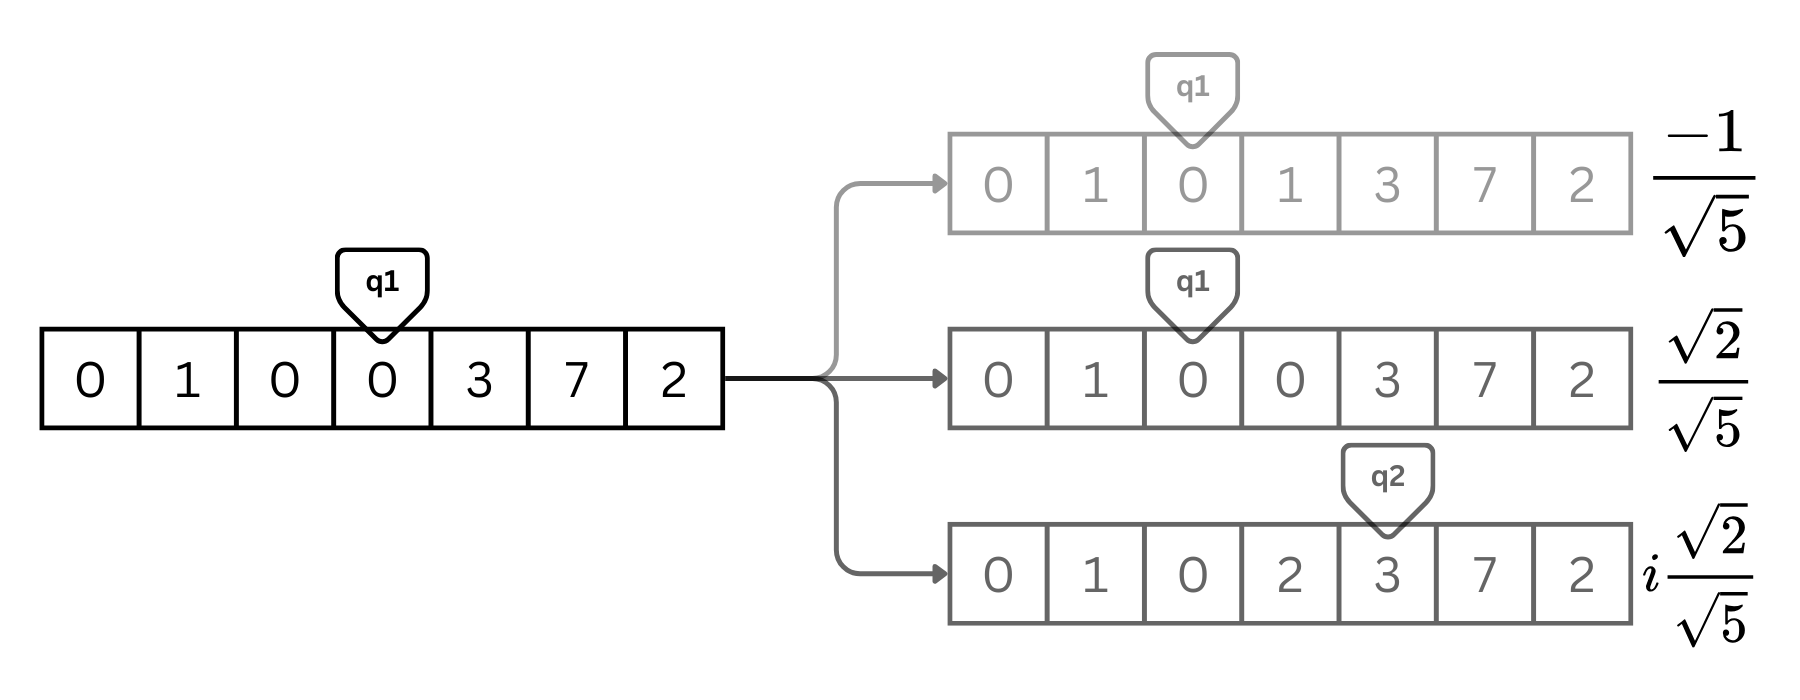
\includegraphics[width=7.5cm]{transition2.png}
		\item<+-> Una pre-macchina di Turing quantistica è una \alert{macchina di Turing quantistica} se \( U_{M} \) è unitario
		\item<+-> \( U_{M} \) unitario se \(\delta\) rispetta certe condizioni
	\end{itemize}
\end{frame}

\section{Funzioni calcolabili quantistiche}

\subsection{PPD e computazioni}

\begin{frame}{\secname}{\subsecname}
	\begin{itemize}
		\item<+-> Una \alert{\foreignlanguage{english}{Partial Probability Distribution} (PPD)} è una funzione \( \mathcal{P} : \mathbb{N} \rightarrow \mathbb{R}_{[0,1]} \) tale che \( \sum_{n \in \mathbb{N}} \mathcal{P} \left ( n \right ) \le 1 \)\par
		Una \alert{\foreignlanguage{english}{Probability Distribution} (PD)} è una \textit{PPD} tale che \( \sum_{n \in \mathbb{N}} \mathcal{P} \left ( n \right ) = 1 \)
		\item<+-> A ogni \( \ket{\phi} \) si può associare una PPD \( \mathcal{P}_{\ket{\phi}} \)\par
		\( \mathcal{P}_{\ket{\phi}} \left ( n \right ) = \) probabilità di \( \ket{\phi} \) di collassare su una configurazione finale con \(n\) simboli \(1\) sul nastro
	\end{itemize}
\end{frame}

\begin{frame}{\secname}{\subsecname}
	\begin{itemize}
		\item<+-> Una \alert{computazione} \(K^{M}_{\ket{\phi}}\) è una sequenza \(\ket{\phi_{i}}\) tale che
		\begin{enumerate}
			\item \(\ket{\phi_{0}} = \ket{\phi}\) è una q-configurazione finale
			\item \(\ket{\phi_{i}} = U_{M}^{i}\ket{\phi}\)
		\end{enumerate}
		\item<+-> A ogni computazione si associa una sequenza di PPD \( \mathcal{P}_{\ket{\phi_{i}}} \)
		\item<+-> La sequenza \(\sum_{n \in \mathbb{N}} \mathcal{P}_{\ket{\phi_{i}}} \left ( n \right )\) è crescente
	\end{itemize}
\end{frame}

\subsection{Definizione}

\begin{frame}{\secname}{\subsecname}
	\begin{itemize}
		\item<1-> Prendiamo in considerazione funzioni di forma \( f : \hiluninorm \left ( \mathbb{N} \right ) \rightarrow PPD \)
		\item<2-> \( \mathcal{P} = \lim_{n \to \infty} \mathcal{P}_{\ket{\phi_{i}}} \) è l'\alert{output calcolato} di M
		\item<2-> Scegliamo una codifica da \( \hiluninorm \left ( \mathbb{N} \right ) \) a \( \hiluninorm \left ( \conf^{init} \right ) \)
		\item<3-> \alert{Funzioni calcolabili quantistiche}: Funzioni \( f : \hiluninorm \left ( \mathbb{N} \right ) \rightarrow PPD \) modellabili da una Macchina di Turing quantistica
	\end{itemize}
\end{frame}

\subsection{Categorie di terminazione}

\begin{frame}{\subsecname}{}
	Una data computazione può
	\begin{enumerate}
		\item<+-> Produrre una \textit{PD} in un numero di passi finito
		\item<+-> Non produrre una \textit{PD} in un numero di passi finito, ma avere una \textit{PD} come \textit{PPD} limite
		\item<+-> Non avere una \textit{PD} come \textit{PPD} limite
	\end{enumerate}
\end{frame}

\section{Conclusione}

\begin{frame}{\secname}{}
	\begin{itemize}
		\item
	\end{itemize}
\end{frame}

\end{document}
